\subsection{The First Marker}

\begin{tikzpicture}
 \node {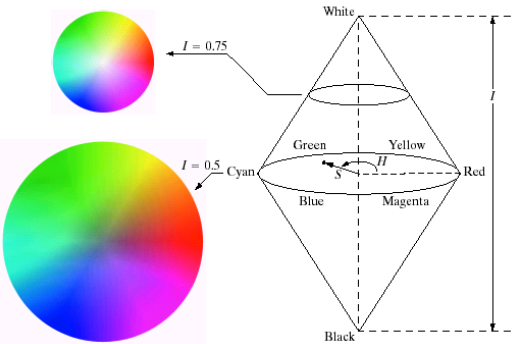
\includegraphics[scale=1]{graphics/hsv} };
 \node[name=hsv, draw, circle, minimum width =5.3cm] at (-4,-1.85) {};
% % % % RED % % % %
% \newcommand{\MinHue}{0} %angle
% \newcommand{\MaxHue}{30}
% \newcommand{\MinSat}{1.6cm} % 0 - 1 => 0 - 2.65
%  \draw (hsv.\MinHue) -- (hsv.center) -- (hsv.\MaxHue);
%  \draw[very thick]   ([shift=(\MinHue:\MinSat)] hsv.center) arc(\MinHue:\MaxHue:\MinSat);
% % % % GREEN % % % %
\newcommand{\MinHue}{70} %angle 
\newcommand{\MaxHue}{145}
\newcommand{\MinSat}{1.6cm} % 0 - 1 => 0 - 2.65
 \draw (hsv.\MinHue) -- (hsv.center) -- (hsv.\MaxHue);
 \draw[very thick]   ([shift=(\MinHue:\MinSat)] hsv.center) arc(\MinHue:\MaxHue:\MinSat);
% % % % BLUE % % % %
% \newcommand{\MinHue}{210} %angle
% \newcommand{\MaxHue}{270}
% \newcommand{\MinSat}{1.6cm} % 0 - 1 => 0 - 2.65
%  \draw (hsv.\MinHue) -- (hsv.center) -- (hsv.\MaxHue);
%  \draw[very thick]   ([shift=(\MinHue:\MinSat)] hsv.center) arc(\MinHue:\MaxHue:\MinSat);

\end{tikzpicture}

